\chapter[Bipolar approval voting]{ Tempering plurality tyranny effects with bipolar approval voting}
\label{sec:21}

\abstract*{}

\abstract{}

\begin{quotation}\emph{The choice of a voting procedure shapes the democracy in which we live}.\\
    -- Baujard A., Gavrel F., Igersheim H., Laslier J.-F. and Lebon I. [BAU-2013p].
\end{quotation}

\section{Bipolar approval voting systems}
\label{sec:21.1}

In the \texttt{votingProfiles} module we provide a \\ \texttt{BipolarApprovalVotingProfile} class for handling voting results where, for each eligible candidate $c$, the voters are invited  to \emph{approve} ($+1$), \emph{disapprove} ($-1$), or \emph{ignore} ($0$) the statement that candidate $c$ should win the election.

File \texttt{bpApVotingProfile.py} Footnote[x] contains such a bipolar approval voting profile concerning 100 voters and 15 eligible candidates \footnote{The file \texttt{bpApVotingProfile.py} may be found in the \texttt{examples} directory of the \Digraph resources.}. We may inspect its content as follows.
\begin{lstlisting}
>>> from votingProfiles import \
...                 BipolarApprovalVotingProfile
>>> bavp = BipolarApprovalVotingProfile('bpApVotingProfile')
>>> bavp
  *------- VotingProfile instance description ------*
    Instance class   : BipolarApprovalVotingProfile
    Instance name    : bpApVotingProfile
    Candidates       : 15
    Voters           : 100
    Attributes       : ['name', 'candidates', 'voters',
                 'approvalBallot', 'netApprovalScores',
                 'ballot']
\end{lstlisting}
Beside the \texttt{candidates} and \texttt{voters} attributes, we discover in Line 11 above the \texttt{approvalBallot} attribute which gathers bipolar approval votes. Its content is the following.
\begin{lstlisting}[caption={Inspecting a bipolar approval ballot},label=list:21.1]
>>> bavp.approvalBallot
  {'v001':
      {'a01': Decimal('0'),
       ...
       'a04': Decimal('1'),
       ...
       'a15': Decimal('0')
      },
   'v002':
       {'a01': Decimal('-1'),
        'a02': Decimal('0'),
        ...
        'a15': Decimal('1')
       },
      ...
   'v100':
     {'a01': Decimal('0'),
      'a02': Decimal('1'),
      ...
      'a15': Decimal('1')
     }
    }
\end{lstlisting}	
Let us denote $A_v$ the set of candidates approved by voter $v$. In the \texttt{approvalBallot} attribute we hence record in fact the bipolar-valued truth characteristic values $r(c \in A_v)$ of the statements that candidate $c$ \emph{is approved} by voter $v$. In Listing \ref{list:21.1} Line 5, we observe for instance that voter 'v001' positively approves candidate 'a04'. And, in Line 10, we see that voter 'v002' negatively approves, i.e. positively disapproves candidate 'a01'.

We may now consult how many approvals or disapprovals each candidate receives.
\begin{lstlisting}
>>> bavp.showApprovalResults()
    Approval results
     Candidate: 'a12' obtains 34 votes
     Candidate: 'a05' obtains 30 votes
     Candidate: 'a03' obtains 28 votes
     Candidate: 'a14' obtains 27 votes
     Candidate: 'a11' obtains 27 votes
     Candidate: 'a04' obtains 27 votes
     Candidate: 'a01' obtains 27 votes
     Candidate: 'a13' obtains 24 votes
     Candidate: 'a07' obtains 24 votes
     Candidate: 'a15' obtains 23 votes
     Candidate: 'a02' obtains 23 votes
     Candidate: 'a09' obtains 22 votes
     Candidate: 'a08' obtains 22 votes
     Candidate: 'a10' obtains 21 votes
     Candidate: 'a06' obtains 21 votes
    Total approval votes: 380
    Approval proportion: 380/1500 = 0.25
>>> bavp.showDisapprovalResults()
    Disapproval results
     Candidate: 'a12' obtains 16 votes
     Candidate: 'a03' obtains 22 votes
     Candidate: 'a09' obtains 23 votes
     Candidate: 'a04' obtains 24 votes
     Candidate: 'a06' obtains 24 votes
     Candidate: 'a13' obtains 24 votes
     Candidate: 'a11' obtains 25 votes
     Candidate: 'a02' obtains 26 votes
     Candidate: 'a07' obtains 26 votes
     Candidate: 'a08' obtains 26 votes
     Candidate: 'a05' obtains 27 votes
     Candidate: 'a10' obtains 27 votes
     Candidate: 'a14' obtains 27 votes
     Candidate: 'a15' obtains 27 votes
     Candidate: 'a01' obtains 32 votes
    Total disapproval votes: 376
    Disapproval proportion: 376/1500 = 0.25
\end{lstlisting}
In Lines 3 and 22 above, we may see that, of all potential candidates, it is Candidate 'a12' who receives the highest number of approval votes (34) and the lowest number of disapproval votes (16). Total number of approval, respectively disapproval, votes approaches more or less a proportion of $25\%$ of the $100 \times 15 = 1500$ potential approval votes. About $50\%$ of the latter remain hence ignored. 

When operating now, for each candidate $c$, the difference between the number of approval and the number of disapproval votes he receives, we obtain per candidate a corresponding \emph{net approval} score; in fact, the bipolar truth characteristic value of the statement ``\emph{candidate c should win the election}''.
\begin{equation}
r(\text{Candidate c should win the election}) \;=\; \sum_v \big(r(c \in A_v)\big)\;.
\end{equation}
These bipolar characteristic values are stored in the \texttt{netApprovalScores} attribute and may be printed out as follows:
\begin{lstlisting}
>>> bavp.showNetApprovalScores()
  Net Approval Scores
     Candidate: 'a12' obtains 18 net approvals
     Candidate: 'a03' obtains 6 net approvals
     Candidate: 'a05' obtains 3 net approvals
     Candidate: 'a04' obtains 3 net approvals
     Candidate: 'a11' obtains 2 net approvals
     Candidate: 'a14' obtains 0 net approvals
     Candidate: 'a13' obtains 0 net approvals
     Candidate: 'a09' obtains -1 net approvals
     Candidate: 'a07' obtains -2 net approvals
     Candidate: 'a06' obtains -3 net approvals
     Candidate: 'a02' obtains -3 net approvals
     Candidate: 'a15' obtains -4 net approvals
     Candidate: 'a08' obtains -4 net approvals
     Candidate: 'a01' obtains -5 net approvals
     Candidate: 'a10' obtains -6 net approvals
\end{lstlisting}
We observe in Line 3 above that Candidate 'a12', with a net approval score of $34 - 16 = 18$, represents indeed the \emph{best approved} candidate for winning the election. With a net approval score of $28-22 = 6$, Candidate 'a03' appears 2nd-best approved. The net approval scores define hence a potentially weak ranking on the set of eligible election candidates, and the winner(s) of the election is(are) determined by the first-ranked candidate(s).

\section{Pairwise comparison of bipolar approval votes}
\label{sec:21.1}


The approval votes of each voter define now on the set of eligible candidates three ordered categories: his approved ($+1$), his ignored ($0$) and his disapproved ($-1$) ones. Within each of these three categories we consider the voter's actual preferences as \emph{not communicated}, i.e. as missing data. This gives for each voter a partially determined strict order which we find in the \texttt{ballot} attribute.
\begin{lstlisting}
 >>> bavp.ballot['v001']['a12']
    {'a02': Decimal('1'), 'a11': Decimal('1'),
     'a14': Decimal('1'), 'a04': Decimal('0'),
     'a06': Decimal('1'), 'a05': Decimal('1'),
     'a12': Decimal('0'), 'a13': Decimal('0'),
     'a15': Decimal('1'), 'a01': Decimal('1'),
     'a08': Decimal('1'), 'a07': Decimal('1'),
     'a09': Decimal('0'), 'a03': Decimal('1'),
     'a10': Decimal('0')}
\end{lstlisting}
For voter 'v001, for instance, the best approved candidate 'a12' is strictly preferred to candidates: 'a01', 'a02', 'a03', 'a05', 'a06', 'a07', 'a08', 'a11', 'a14' and '15'. No candidate is preferred to 'a12' and the comparison with 'a04', 'a09', 'a10' and 'a13' is not communicated, hence indeterminate. Mind by the way that the reflexive comparison of 'a12' with itself is, as usual, is ignored, i.e. indeterminate. Each voter $v$ defines thus a partially determined transitive strict preference relation denoted $\succ_v$ on the eligible candidates.

For each pair of eligible candidates, we aggregate the previous individual voter's preferences into a truth characteristic of the statement: ``candidate $x$ is \emph{better approved than} candidate $y$'', denoted $r(x \succ y)$:
\begin{equation}
  r(x \succ y)\;=\; \sum_v \big(\,r(x \succ_v y)\, \big)\;.
\end{equation}  

We say that candidate $x$ is \emph{better approved than} Candidate $y$ when $r(x \succ y)\;>\;0$, i.e. there is a majority of voters who approve \emph{more} and disapprove \emph{less} $x$ than $y$. Vice-versa, we say that candidate $x$ is \emph{not} better approved than candidate $y$ when $r(x \succ y)\;<\;0$, i.e. there is a majority of voters who disapprove more and approve less $x$ than $y$. This computation is achieved with the \texttt{MajorityMarginsDigraph} constructor.
\begin{lstlisting}
>>> from votingProfiles import MajorityMarginsDigraph
>>> m = MajorityMarginsDigraph(bavp)
>>> m
  *------- Digraph instance description ------*
    Instance class      : MajorityMarginsDigraph
    Instance name       : rel_bpApVotingProfile
    Digraph Order       : 15
    Digraph Size        : 97
    Valuation domain    : [-100.00;100.00]
    Determinateness (%) : 52.55
    Attributes          : ['name', 'actions',
               'criteria','ballot',
               'valuationdomain', 'relation',
               'order', 'gamma', 'notGamma']
\end{lstlisting}
The resulting digraph $m$ contains 97 positively validated relations (see Line 8 above) and (see Line 9) for all pairs $(x,y)$ of eligible candidates, $r(x \succ y)$ takes value in an valuation range from $-100.00$ (all voters opposed) to $+100.00$ (unanimously supported).

We may inspect these pairwise $r(x \succ y)$ values in a browser view: 
\begin{lstlisting}
>>> m.showHTMLRelationTable(relationName='r(x > y)')
\end{lstlisting}
\begin{figure}[h]
%\sidecaption
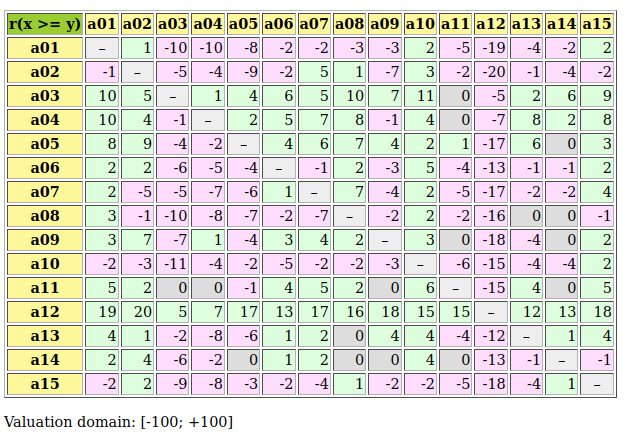
\includegraphics[width=11cm]{Figures/majMargAV.png}
\caption{The bipolar-valued pairwise majority margins} 
\label{fig:21.1}       % Give a unique label
\end{figure}

It gets easily apparent that candidate 'a12' is a \Condorcet winner, i.e. the candidate who beats all the other candidates and, with the given voting profile $gavp$, should without doubt win the election. This strongly confirms the first-ranked result obtained with the previous net approval scoring. 

Let us eventually compute, with the help of the \NetFlows ranking rule, a linear ranking of the 15 eligible candidates and compare the result with the net approval scores ranking.
\begin{lstlisting}[caption={Comparing the net approval and the \NetFlows rankings},label=list:21.2]
>>> from linearOrders import NetFlowsOrder
>>> nf = NetFlowsOrder(m,Comments=True)
>>> print('NetFlows versus Net Approval Ranking')
>>> print('Candidate\tNetFlows score\tNet Approval score')
>>> for item in nf.netFlows:
...     print( '%9s\t  %+.3f\t %+.1f' %\
...	        (item[1], item[0],\
...              bavp.netApprovalScores[item[1]]) ) 
    NetFlows versus Net Approval Ranking
    Candidate	NetFlows score	Net Approval score
      'a12'	  +410.000	 +18.0
      'a03'	  +142.000	  +6.0
      'a04'	   +98.000	  +3.0
      'a05'	   +54.000	  +3.0
      'a11'	   +34.000	  +2.0
      'a09'	   -16.000	  -1.0
      'a14'	   -20.000	  +0.0
      'a13'	   -22.000	  +0.0
      'a06'	   -50.000	  -3.0
      'a07'	   -74.000	  -2.0
      'a02'	   -96.000	  -3.0
      'a08'	   -102.000	  -4.0
      'a15'	   -110.000	  -4.0
      'a10'	   -122.000	  -6.0
      'a01'	   -126.000	  -5.0
\end{lstlisting}
In Listing \ref{list:21.2} we may notice that the \NetFlows rule delivers a ranking that is very similar to the one previously obtained with the corresponding \emph{Net Approval} scores. Only minor inversions do appear, like in the midfield, where candidate 'a09' advances before candidates 'a13' and a14' (see Line 16) , and 'a6' and 'a07' swap their positions 9 and 10 (see Line 19). And, the two last-ranked candidates 'a10' and 'a01' also swap their positions.

This confirms again the pertinence of the net approval scoring approach for finding the winner in a bipolar approving voting system. Yet, voting by approving ($+1$), disapproving ($-1$) or ignoring ($0$) eligible candidates, may also be seen as a performance evaluation of the eligible candidates on a $\{-1, 0, 1\}$-graded ordinal scale.

\section{Three-valued evaluative voting system}
\label{sec:21.2}

Following such an epistemic perspective, we may effectively convert the given \texttt{BipolarApprovalVotingProfile} instance into\\ a \texttt{PerformanceTableau} instance, so as to get access to a corresponding outranking decision aiding approach.

Mind that, contrary to the majority margins of the ``\emph{better approved than}'' relation, all voters consider now the approved candidates to be all equivalent ($+1$). Same is true for the disapproved ($-1$), respectively the ignored ($0$) candidates. The voter's marginal preferences model this time a complete preorder with three equivalence classes. 

From the saved file \texttt{AVPerfTab.py} (see Line 1 below), we may construct an outranking relation on the eligible candidates with our \\ standard \texttt{BipolarOutrankingDigraph} constructor. The semantics of this outranking relation are the following:
\begin{itemize}
\item We say that Candidate $x$ \emph{outranks} Candidate $y$ when there is a majority of voters who consider $x$ \emph{at least as well evaluated as} $y$ (see Line3 below);
\item We say that Candidate $x$ is \emph{outranked by} Candidate $y$ when there is a majority of voters who consider $x$ \emph{not at least as well evaluated as} $y$.
\end{itemize}
\begin{lstlisting}[caption={Computing the outranking digraph},label=list:21.3]
>>> bavp.save2PerfTab(fileName='AVPerfTab',valueDigits=0)
  *--- Saving as performance tableau in AVPerfTab.py ---*
>>> from outrankingDigraphs import\
...                         BipolarOutrankingDigraph
>>> odg = BipolarOutrankingDigraph('AVPerfTab')
>>> odg
  *------- Object instance description ------*
    Instance class       : BipolarOutrankingDigraph
    Instance name        : rel_AVPerfTab
    Actions              : 15
    Criteria             : 100
    Size                 : 210
    Determinateness (%)  : 69.29
    Valuation domain     : [-1.00;1.00]
    Attributes           : ['name', 'actions', 'order,
                       'criteria', 'evaluation', 'NA',
                       'valuationdomain', 'relation',
                       'gamma', 'notGamma', ...]
\end{lstlisting}
The size ($210 = 15 \times 14$) of the resulting outranking digraph $odg$, shown in Listing \ref{list:21.3} Line 11 above, reveals that the corresponding ``\emph{at least as good evaluated as}'' relation models actually a trivial \emph{complete} digraph. All candidates appear to be \emph{equally} at least as well evaluated and the strict ``\emph{better evaluated than}'' (codual) outranking digraph becomes in fact empty. The converted performance tableau does apparently not contain sufficiently discriminatory performance evaluations for supporting any strict preference situations.

Yet, we may nevertheless try to apply again the \NetFlows ranking rule to this complete outranking digraph $odg$ and print side by side the corresponding \NetFlows scores and the previous Net Approval scores. 
\begin{lstlisting}[caption={Comparing the \NetFlows and the Net Approval rankings},label=list:21.4]
>>> from linearOrders import NetFlowsOrder
>>> nf = NetFlowsOrder(odg)
>>> print('NetFlows versus Net Approval Ranking')
>>> print('Candidate\tNetFlows Score\tNet Approval Score')
>>> for item in nf.netFlows:
...     print('%9s\t  %+.3f\t %+.0f' %\
...         ('\'',item[1],'\'', item[0],\
...          bavp.netApprovalScores[item[1]]) )  
    NetFlows versus Net Approval Ranking
    Candidate    NetFlows score	Net Approval score
       'a12	  +4.100	   +18.0
       'a03	  +1.420	    +6.0
       'a04	  +0.980	    +3.0
       'a05	  +0.540	    +3.0
       'a11	  +0.340	    +2.0
       'a09	  -0.160	    -1.0
       'a14	  -0.200	    +0.0
       'a13	  -0.220	    +0.0
       'a06	  -0.500	    -3.0
       'a07	  -0.740	    -2.0
       'a02	  -0.960	    -3.0
       'a08	  -1.020	    -4.0
       'a15	  -1.100	    -4.0
       'a10	  -1.220	    -6.0
       'a01	  -1.260	    -5.0
\end{lstlisting}
Despite its apparent poor strict preference discriminating power, we obtain in Listing \ref{list:21.4} here \NetFlows scores that are directly proportional (divided by $100$) to the scores obtained with the \emph{better approved than} majority margins digraph $m$ (see Listing \ref{list:21.2}).

Encouraged by this positive result, we may furthermore try to compute as well a best choice recommendation.
\begin{lstlisting}[caption={Computing a best social choice recommendation},label=list:21.5]
>>> odg.showBestChoiceRecommendation(CoDual=True)
  Rubis best choice recommendation(s) (BCR)
   (in decreasing order of determinateness)   
   Credibility domain: [-1.00,1.00]
  === >> ambiguous best choice(s) 
   * choice        : ['a01','a02','a03','a04','a05',
                      'a06','a07','a08','a09','a10',
                      'a11','a12','a13','a14','a15']
    independence   : 0.06
    dominance      : 1.00
    absorbency     : 1.00
    covering (%)   : 100.00
    determinateness (%) : 61.13
    - most credible action(s) = {
        'a12': 0.44, 'a03': 0.34, 'a04': 0.30,
        'a14': 0.28, 'a13': 0.24, 'a06': 0.24,
        'a11': 0.20, 'a10': 0.20, 'a07': 0.20,
        'a01': 0.20, 'a08': 0.18, 'a05': 0.18,
        'a15': 0.14, 'a09': 0.14, 'a02': 0.06, }
   === >> ambiguous worst choice(s)
    * choice        : ['a01','a02','a03','a04','a05',
                      'a06','a07','a08','a09','a10',
                      'a11','a12','a13','a14','a15']
     independence   : 0.06
     dominance      : 1.00
     absorbency     : 1.00
     covered (%)    : 100.00
     determinateness (%) : 63.73
     - most credible action(s) = {
         'a13': 0.36, 'a06': 0.36, 'a15': 0.34,
         'a01': 0.34, 'a08': 0.32, 'a07': 0.30,
         'a02': 0.30, 'a14': 0.28, 'a11': 0.28,
         'a09': 0.28, 'a04': 0.26, 'a10': 0.24,
         'a05': 0.20, 'a03': 0.20, 'a12': 0.06, }
\end{lstlisting}
The strict outranking digraph $(\sim (-odg))$ being actually $empty$, we obtain a unique \emph{ambiguous} --best as well as last-- choice recommendation which trivially retains all fifteen candidates (see Listing \ref{list:21.5} Lines 6-8 above). Yet, the bipolar-valued best choice membership characteristic vector reveals that, among all the fifteen potential winners, it is indeed Candidate 'a12' the most credible one with a $72\%$ majority of voters' support (see Line 15, $(0.44 + 1.0)/2\;=\; 0.72$); followed by Candidate 'a03' ($67\%$) and Candidate 'a04' ($65\%$). Similarly, Candidates 'a13' and 'a06' represent the most credible losers with a $68\%$ majority voters' support (Line 30).

We observe here empirically that \emph{evaluative} voting systems, using three-valued ordinal performance scales, match closely a corresponding bipolar approval voting systems. The latter voting system models, however, more faithfully the very preferential information that is expressed with \emph{approved}, \emph{disapproved} or \emph{ignored} statements. The corresponding evaluation on a three-graded scale, being value (numbers) based, cannot express the fact that in bipolar approval voting systems there is no preferential information given concerning the pairwise comparison of all approved, respectively disapproved or ignored candidates.

Let us finally illustrate how bipolar approval voting systems may favour multipartisan supported candidates. We shall therefore compare \emph{bipolar approval} versus \emph{uninominal plurality} election results when considering a highly divisive and partisan political context.
 
\section{Favouring multipartisan candidates}
\label{sec:21.3}

In modern democracy, politics  are largely structured by political parties and activists movements. Let us so consider a bipolar approval voting profile $dvp$ where the random voter behaviour is simulated from two pre-electoral polls concerning a political scene with essentially two major competing parties, like the one existing in the US.
\begin{lstlisting}[caption={A random bipolar approval voting profile in a divisive political context},label=list:21.6]
>>> dvp = RandomBipolarApprovalVotingProfile(\
...                numberOfCandidates=15,
...                numberOfVoters=100,
...                approvalProbability=0.25,
...                disapprovalProbability=0.25,
...                WithPolls=True,
...                partyRepartition=0.5,
...                other=0.05,
...                DivisivePolitics=True,
...                seed=200)
>>> dvp.showRandomPolls()
  Random repartition of voters
  Party-1 supporters : 45 (45.00%)
  Party-2 supporters : 49 (49.00%)
  Other voters       : 6 (06.00%)
  *---------------- random polls -----------------
  Party-1(45.0%) | Party-2(49.0%) |   expected  
  ------------------------------------------------
  'a05' : 24.10% | 'a07' : 24.10% | 'a07' : 11.87%
  'a14' : 23.48% | 'a10' : 23.48% | 'a10' : 11.60%
  'a03' : 15.13% | 'a01' : 15.13% | 'a05' : 10.91%
  'a12' : 07.55% | 'a04' : 07.55% | 'a14' : 10.67%
  'a08' : 07.11% | 'a09' : 07.11% | 'a01' : 07.67%
  'a15' : 04.37% | 'a13' : 04.37% | 'a03' : 07.09%
  'a11' : 03.99% | 'a02' : 03.99% | 'a04' : 04.55%
  'a06' : 03.80% | 'a06' : 03.80% | 'a09' : 04.49%
  'a02' : 02.79% | 'a11' : 02.79% | 'a12' : 04.32%
  'a13' : 02.63% | 'a15' : 02.63% | 'a08' : 04.30%
  'a09' : 02.24% | 'a08' : 02.24% | 'a06' : 03.57%
  'a04' : 01.89% | 'a12' : 01.89% | 'a13' : 03.32%
  'a01' : 00.57% | 'a03' : 00.57% | 'a15' : 03.25%
  'a10' : 00.20% | 'a14' : 00.20% | 'a02' : 03.21%
  'a07' : 00.14% | 'a05' : 00.14% | 'a11' : 03.16%
\end{lstlisting}   
In Listing \ref{list:21.6}, the divisive political situation is reflected by the fact that Party-1 and Party-2 supporters show strict reversed preferences. The leading candidates of Party-1 ('a05' and 'a14') are last choices for Party-2 supporters and, Candidates 'a07' and 'a10', leading candidates for Party-2 supporters, are similarly the least choices for Party-1 supporters.

No clear winner may be guessed from these pre-election polls. As Party-2 shows however slightly more supporters than Party-1, the expected winner in an uninominal plurality or instant-runoff voting system will be Candidate 'a07', i,e, the leading candidate of majority Party-2 (see below).
\begin{lstlisting}
>>> dvp.computeSimpleMajorityWinner()
  ['a07']
>>> dvp.computeInstantRunoffWinner()
  ['a07']
\end{lstlisting}

Now, in a corresponding bipolar approval voting system, Party-1 supporters will usually approve their leading candidates and disapprove the leading candidates of Party-2. Vice versa, Party-2 supporters will usually approve their leading candidates and disapprove the leading candidates of Party-1. Let us consult the resulting approval votes per candidate.
\begin{lstlisting}
>>> dvp.showApprovalResults()
     Candidate: 'a07' obtains 30 votes
     Candidate: 'a10' obtains 28 votes
     Candidate: 'a05' obtains 28 votes
     Candidate: 'a01' obtains 28 votes
     Candidate: 'a03' obtains 26 votes
     Candidate: 'a02' obtains 26 votes
     Candidate: 'a12' obtains 25 votes
     Candidate: 'a14' obtains 24 votes
     Candidate: 'a13' obtains 24 votes
     Candidate: 'a09' obtains 21 votes
     Candidate: 'a04' obtains 21 votes
     Candidate: 'a08' obtains 19 votes
     Candidate: 'a06' obtains 17 votes
     Candidate: 'a15' obtains 15 votes
     Candidate: 'a11' obtains 12 votes
    Total approval votes: 344
    Approval proportion: 344/1500 = 0.23
\end{lstlisting}
When considering only the approval votes, we find confirmed above that the leading candidate of Party-2 obtains in this simulation a plurality of approval votes. In uninominal plurality or instant-runoff voting systems, this candidate wins hence the election, quite to the despair of Party-1 supporters. As a foreseeable consequence, this election result will be more or less aggressively contested which leads to a loss of popular trust in democratic elections and institutions.

If we look however on the corresponding disapprovals, we discover that, not surprisingly, the leading candidates of both parties collect by far the highest number of disapproval votes. 
\begin{lstlisting}
>>> dvp.showDisapprovalResults()
     Candidate: 'a02' obtains 14 votes
     Candidate: 'a04' obtains 14 votes
     Candidate: 'a13' obtains 14 votes
     Candidate: 'a06' obtains 15 votes
     Candidate: 'a09' obtains 15 votes
     Candidate: 'a08' obtains 16 votes
     Candidate: 'a11' obtains 16 votes
     Candidate: 'a15' obtains 18 votes
     Candidate: 'a12' obtains 20 votes
     Candidate: 'a01' obtains 29 votes
     Candidate: 'a03' obtains 30 votes
     Candidate: 'a10' obtains 37 votes
     Candidate: 'a07' obtains 44 votes
     Candidate: 'a14' obtains 45 votes
     Candidate: 'a05' obtains 49 votes
    Total disapproval votes: 376
    Disapproval proportion: 376/1500 = 0.25
\end{lstlisting}
Balancing now approval against disapproval votes will favour the moderate, bipartisan supported, candidates.
\begin{lstlisting}
>>> dvp.showNetApprovalScores()
    Net Approval Scores
     Candidate: 'a02' obtains 12 net approvals
     Candidate: 'a13' obtains 10 net approvals
     Candidate: 'a04' obtains 7 net approvals
     Candidate: 'a09' obtains 6 net approvals
     Candidate: 'a12' obtains 5 net approvals
     Candidate: 'a08' obtains 3 net approvals
     Candidate: 'a06' obtains 2 net approvals
     Candidate: 'a01' obtains -1 net approvals
     Candidate: 'a15' obtains -3 net approvals
     Candidate: 'a11' obtains -4 net approvals
     Candidate: 'a03' obtains -4 net approvals
     Candidate: 'a10' obtains -9 net approvals
     Candidate: 'a07' obtains -14 net approvals
     Candidate: 'a14' obtains -21 net approvals
     Candidate: 'a05' obtains -21 net approvals
\end{lstlisting}
Candidate 'a02', appearing in the pre-electoral polls in the midfield (in position 7 for Party-2 and in position 9 for Party-1 supporters, see Listing \ref{list:21.6}), shows indeed the highest net approval score. Second highest net approval score obtains Candidate 'a13', in  position 6 for Party-2 and in position 10 for Party-1 supporters.

Fig. \ref{fig:21.2}, showing the \NetFlows ranked relation table of the ``\emph{better approved than}'' majority margins digraph, confirms below this net approval scoring result.
\begin{lstlisting}
>>> m = MajorityMarginsDigraph(dvp)
>>> m.showHTMLRelationTable(\
...      actionsList=m.computeNetFlowsRanking(),
...      relationName='r(x > y)')
\end{lstlisting}	   
\begin{figure}[h]
%\sidecaption
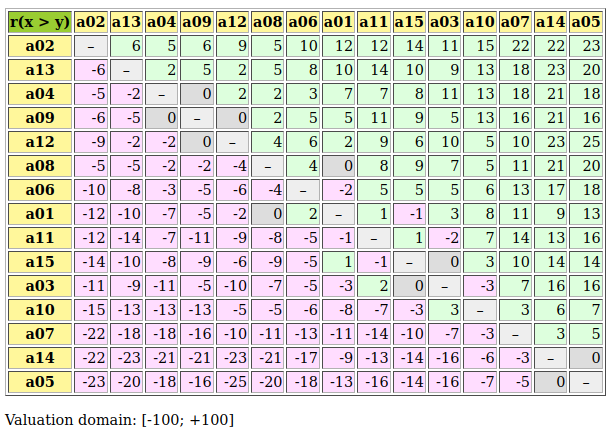
\includegraphics[width=11cm]{Figures/majMargDAV.png}
\caption{The pairwise \emph{better approved than} majority margins} 
\label{fig:21.2}       % Give a unique label
\end{figure}
Candidate 'a02' appears indeed \emph{better approved than} any other candidate (\Condorcet winner); and, the leading candidates of Party-1, 'a05' and 'a14', are \emph{less approved than} any other candidates (weak \Condorcet losers).
\begin{lstlisting}
>>> m.computeCondorcetWinners()
  ['a02']
>>> m.computeWeakCondorcetLosers()
  ['a05','a14']
\end{lstlisting}

We see this result furthermore confirmed when computing the corresponding best, respectively worst choice recommendation.    
\begin{lstlisting}
>>> m.showBestChoiceRecommendation()
  Rubis best choice recommendation(s) (BCR)
   (in decreasing order of determinateness)   
   Credibility domain: [-100.00,100.00]
   === >> potential best choice(s)
    * choice              : ['a02']
      independence        : 100.00
      dominance           : 5.00
      absorbency          : -23.00
      covering (%)        : 100.00
      determinateness (%) : 52.50
      - most credible action(s) = { 'a02': 5.00, }
   === >> potential worst choice(s) 
    * choice              : ['a05', 'a14']
      independence        : 0.00
      dominance           : -23.00
      absorbency          : 5.00
      covered (%)         : 100.00
      determinateness (%) : 50.00
      - most credible action(s) = { }
\end{lstlisting}
Candidate 'a02', being actually a \Condorcet winner, gives an initial prekernel of digraph $m$, whereas Party-1 leading Candidates 'a05' and 'a14', both being weak \Condorcet losers, give together a terminal prekernel. They hence represent our \emph{best choice}, respectively, \emph{worst choice} recommendations for winning this simulated election.

Let us conclude by predicting that, for leading political candidates in an aggressively divisive political context, the perspective to easily fail election with bipolar approval voting systems, might or will induce a change in the usual way of running electoral campaigns. Political parties and politicians, who avoid aggressive competitive propaganda and instead propose multipartisan collaborative social choices, will be rewarded with better election results than any kind of extremism. It could mean the end of sterile political obstructions and war like electoral battles. \emph{Let's do it !}.

It is worthwhile noticing again the essential structural and computational role, the ignored value is again playing in bipolar approval voting systems. This epistemic and logical \emph{neutral} term is needed indeed for handling in a consistent and efficient manner \emph{not communicated votes} and/or \emph{indeterminate} preferential statements.
 
